%\chapter{Desenvolvimento do Jogo}
\chapter{Resultados Parciais}
\label{chap:des}

Neste capítulo é apresentado como se deu a execução da metodologia adotada neste trabalho. Na sequência é descrito como as personas foram definidas, a ideação do jogo e a definição de aspectos técnicos da engenharia de software.

\section{Ciclo de vida do jogo}

Como apresentado no Capítulo \ref{chap:Metodo}, o desenvolvimento do jogo PersonaDesignGame inicia-se a partir revisão da literatura e definição do escopo. Esse processo segue se apoiando no \textit{Playcentric Design Process} juntamente com algumas diretrizes da Engenharia de software. Na revisão da literatura, além da base de conhecimento para realização do projeto, foi possível levantar alguns requisitos a partir da identificação dos trabalhos sobre jogos em IHC mencionados no Referencial Teórico, Capítulo \ref{chap:ref}, Seção \ref{sec:trab_cor}. 

Na etapa de definição escopo foi elaborado um \textit{survey}, no qual foi desenvolvido e aplicado um questionário de pesquisa, que teve como objetivo identificar o público-alvo e elicitar mais alguns requisitos. O relatório do \textit{survey} é descrito no Apêndice \ref{ap:questionario} assim como o próprio questionário. Para finalizar essa etapa e fechar o escopo foram elaboradas personas, estas guiaram a definição, especificação e validação dos requisitos identificados.

O elenco de personas criado também participou de todo o processo de design ao longo do projeto. Como persona primária, o arquétipo alvo do projeto, temos Victor Matheus Farias; como persona secundária temos o Afonso de Souza Queiroz; como persona suplementar temos a Natália Figueiredo; e por fim temos a anti-persona Rafael Medeiros. Todas elas estão detalhadas no Apêndice \ref{ap:persona}.%, assim como o processo de sua construção.

A partir das personas definidas, foram elaboradas a ideia base do jogo, definidos os requisitos funcionais, não funcionais e as metas de experiência do jogador, e elaborado o protótipo de papel (Apêndice \ref{ap:proto_papel}). Isso tudo está descrito no Game Design Document, Seção \ref{sec:gdd} e no Technical Design Document, Seção \ref{sec:tdd}.

\section{Game Design Document}
\label{sec:gdd}
Nesta seção é apresentado o GDD, documento no qual estão especificados as características gerais do jogo, \textit{gameplay}, mecânica e fluxo do jogo, regras, os seus elementos, \textit{storyboard} e identidade visual. Este artefato é evolutivo, sendo incrementado e sofrendo alterações ao longo do projeto.

\subsection{Características Gerais}
O jogo elaborado neste trabalho é o PersonaDesignGame, o jogo de aprendizado sobre personas. Este é classificado como um jogo de gênero educacional, de perguntas e respostas. Trata-se de um jogo 2D, com um perspectiva em primeira pessoa, no qual o modo de jogo é \textit{single player}.

O PersonaDesignGame  tem como seus jogadores-alvo, alunos de graduação e pós graduação em cursos da área de Ciência da Computação. Neste jogo o estudante irá aprender o conteúdo sobre a técnica de personas, exercitá-lo e por fim ter um exemplo prático de como se construir um persona.

\subsection{Gameplay}

O objetivo do jogo é responder corretamente todas a perguntas. Para isso o jogador terá de executar a seguinte mecânica:

\begin{enumerate}
    \item ao iniciar a partida o jogador receberá um trecho do conteúdo sobre personas;
    \item em seguida é apresentada um questão referentes ao conteúdo disponibilizado;
    \item caso responda corretamente o jogador passa para a próxima pergunta; e
    \item caso responda errado ele deve repetir a questão.
\end{enumerate}

O jogo segue uma regra básica: só é liberado um novo conteúdo após a resolução correta de todas as questões referentes ao último conteúdo liberado. As questões são agrupadas por fases, e cada fase têm grupos menores de questões, as etapas. Ao todo são duas fases que contemplam os aspectos gerais sobres as pesonas e sobre a construção de personas, como é descrito a seguir:

\begin{itemize}
    \item \textbf{Fase 1:}
    
    \textbf{Tema:} Aspectos Gerais sobre Pesonas.
    
    \textbf{Tipo de Questão:} Verdadeiro ou Falso; Múltipla Escolha.
    
    \item  \textbf{Fase 2:} 
    
    \textbf{Tema:} Aspectos da Construção Pesonas.
    
    \textbf{Tipo de Questão:} Verdadeiro ou Falso; Múltipla Escolha.
    
\end{itemize}

Ao longo das questões algumas dicas estarão habilitadas para que o jogador possa relembrar de algum termo sem precisar voltar ao conteúdo apresentado anteriormente. Durante a resolução das questões, \textit{cards} de característica de personas podem ser coletados como recompensa. Segue na Figura \ref{Fig:game_flow.png} o fluxo do jogo:

\begin{figure}[htbp]
	\centering
		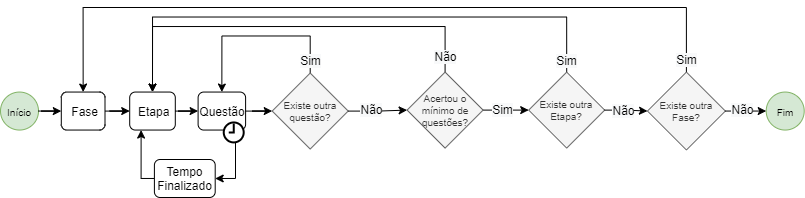
\includegraphics[keepaspectratio=true,scale=0.56]{figuras/game_flow.png}
		\caption{Fluxo da Partida do Jogo - Próprio Autor}
	\label{Fig:game_flow.png}
\end{figure}

\subsection{Elementos do Jogo}

O jogo PersonaDesignGame conta com três ambientes. O primeiro é o Menu Inicial no qual é centralizado o acesso às demais funcionalidades, ambientes e ações do jogo. Outro ambiente é a própria partida do jogo, onde o jogador pode iniciar a resolução das questões.

Existe também o ambiente Resumos, no qual o jogador tem acesso ao conteúdo sobre as personas. Por fim no ambiente Personas são apresentados as personas e seus respectivos \textit{cards}.

Os \textit{cards} estão relacionados aos dados do público-alvo e são coletados no processo de design para se elaborar as personas. Os \textit{cards} elaborados são os seguintes:

\begin{itemize}
    \item Identidade;
    \item Objetivos;
    \item Habilidades;
    \item Tarefas;
    \item Relacionamento;
    \item Requisitos; e
    \item Expectativas.
\end{itemize}
% especificar onde cada card é liberado

% \subsection{Identidade Visual}

% \subsection{Protótipo}


\section{Technical Design Document}
\label{sec:tdd}
Nesta seção é apresentado o TDD, documento no qual estão especificados os elementos técnicos relacionados ao jogo digital. Aqui estão especificados os requisitos elicitados, as técnicas de modelagem usadas, a arquitetura do software, as características do sistema e a configuração do ambiente de desenvolvimento. Este artefato é um planejamento para a execução do projeto, normalmente ele é alterado ao longo do projeto

\subsection{Requisitos}

Nesta subseção são apresentados os requisitos definidos para o projeto. São eles, requisitos funcionais, requisitos não funcionais e as metas de experiência do jogador. 
% Os requisitos funcionais e não funcionais estão apresentados como "requisitos épicos", num alto grau de abstração. Uma modelagem trazendo um granularidade menor para os requisitos será desenvolvida. A modelagem irá consistir em "Épicos", "Requisitos", "Histórias de Usuário", "Tarefas" e "Critérios de Aceitação". Este tipo de modelagem traz uma perspectiva de rastreabilidade dos requisitos e auxilia na fase de implementação. 

Na Tabela \ref{tab:Table_rf}, temos os requisitos funcionais do jogo. Estes descrevem as funções que o software deve executar. Eles também são conhecidos como recursos \cite{Bourque_2014}. 

% Épicos: Conteúdo didático, Dinânima de questões, Fluxo do jogo, Fluxo da partida e Personas


% Descrever a rastreabilidade de cada requisito (?)
\begin{table}[htbp]
    \centering
\caption{\textcolor{textmodified}{Requisitos Funcionais}}
\label{tab:Table_rf}
\begin{tabular}{|p{0.9cm}|p{2.5cm}|p{9.3cm}|p{1.9cm}|}
\hline
\textcolor{textmodified}{ID}   & \textcolor{textmodified}{Épico}          & \textcolor{textmodified}{Descrição} & \textcolor{textadded}{Priorização}                                                                                                                                                                                                               \\ \hline
\textcolor{textmodified}{RF01} & \textcolor{textmodified}{Conteúdo didático} &\textcolor{textmodified}{O jogo deve dispor do conteúdo sobre personas de forma objetiva, em resumos e dicas nas questões.} & \textcolor{textadded}{SHOULD} \\ \hline

\textcolor{textmodified}{RF02} & \textcolor{textmodified}{Dinâmica das questões}        & \textcolor{textmodified}{As questões devem conter o texto da pergunta.} & \textcolor{textadded}{MUST}  \\ \hline

\textcolor{textmodified}{RF03} & \textcolor{textmodified}{Dinâmica das questões}        & \textcolor{textmodified}{As questões devem permitir o usuário a escolher a resposta entre as alternativas de múltipla escolha ou de verdadeiro ou falso.} & \textcolor{textadded}{MUST}  \\ \hline

\textcolor{textmodified}{RF04} & \textcolor{textmodified}{Dinâmica das questões}        & \textcolor{textmodified}{Deve ser possível confirmar a resposta selecionada antes de enviá-la para validação.} & \textcolor{textadded}{COULD}  \\ \hline

\textcolor{textmodified}{RF05} & \textcolor{textmodified}{Resposta ao Usuário}       & \textcolor{textmodified}{O jogo deve validar a resposta e fornecer \textit{feedbacks} ao usuário de resposta certa ou errada.} & \textcolor{textadded}{MUST}  \\ \hline   

\textcolor{textmodified}{RF06} & \textcolor{textmodified}{Resposta ao Usuário}       & \textcolor{textmodified}{Caso o jogador tenha errado uma questão, o jogo deve apresentar a resposta correta.} & \textcolor{textadded}{MUST}  \\ \hline

\textcolor{textmodified}{RF07} & \textcolor{textmodified}{Resposta ao Usuário}       & \textcolor{textmodified}{Caso o jogador tenha acertado uma questão, o jogo deve apresentar uma mensagem de congratulação ou uma recompensa, com a explicação da resposta correta.} & \textcolor{textadded}{SHOULD}  \\ \hline

\textcolor{textmodified}{RF08} & \textcolor{textmodified}{Fluxo da partida}          & \textcolor{textmodified}{O jogo deve manter bloqueada uma etapa da fase até que a etapa anterior seja concluída.} & \textcolor{textadded}{MUST} \\ \hline

\textcolor{textmodified}{RF09} & \textcolor{textmodified}{Fluxo da partida}          & \textcolor{textmodified}{O jogo deve permitir o usuário iniciar uma partida selecionando a etapa da fase que ele deseja jogar.} & \textcolor{textadded}{MUST} \\ \hline

\textcolor{textmodified}{RF10} & \textcolor{textmodified}{Fluxo da partida}            & \textcolor{textmodified}{Ao selecionar uma etapa da fase o jogador deve confirmar se ele deseja iniciá-la.} & \textcolor{textadded}{COULD} \\ \hline

\textcolor{textmodified}{RF11} & \textcolor{textmodified}{Fluxo da partida}            & \textcolor{textmodified}{O jogo deve permitir o usuário sair da partida.} & \textcolor{textadded}{COULD} \\ \hline

\textcolor{textadded}{RF12} & \textcolor{textadded}{Fluxo da partida}            & \textcolor{textadded}{O jogo deve permitir o usuário progredir ao responder as questões corretamente.} & \textcolor{textadded}{MUST} \\ \hline

\textcolor{textadded}{RF13} & \textcolor{textadded}{Fluxo da partida}            & \textcolor{textadded}{O jogo deve fornecer um tempo limite para que o jogador responda as questões de uma etapa.} & \textcolor{textadded}{SHOULD} \\ \hline

\textcolor{textmodified}{RF14} & \textcolor{textmodified}{Fluxo de jogo}            & \textcolor{textmodified}{O jogo deve permitir o usuário a visualizar as fases e etapas, o conteúdo didático e a área de recompensas.} & \textcolor{textadded}{MUST} \\ \hline

\textcolor{textmodified}{RF15} & \textcolor{textmodified}{Fluxo de jogo}             & \textcolor{textmodified}{O jogo deve salvar o progresso do jogador durante a sessão.} & \textcolor{textadded}{SHOULD} \\ \hline

\textcolor{textmodified}{RF16} & \textcolor{textmodified}{Recompensas}                 & \textcolor{textmodified}{O jogo deve salvar os cards de personas coletados durante as partidas do jogo. E deve ser possível visualizá-las em suas respectivas áreas de recompensa.} & \textcolor{textadded}{SHOULD} \\ \hline

\textcolor{textadded}{RF17} & \textcolor{textadded}{Recompensas}                 & \textcolor{textadded}{O jogo deve permitir o jogador a ganhar medalhas como recompensa por completar desafios do jogo.} & \textcolor{textadded}{SHOULD} \\ \hline

\textcolor{textadded}{RF18} & \textcolor{textadded}{Recompensas}                 & \textcolor{textadded}{O jogo deve possuir medalhas de recompensa de ouro, prata e bronze. Ouro é o maior e bronze é o menor desempenho dentro do jogo.} & \textcolor{textadded}{COULD} \\ \hline

\end{tabular}
\end{table}


Na sequência temos na Tabela \ref{tab:Table_rnf} os requisitos não funcionais do jogo numa visão macro. Eles atuam para restringir a solução e também podem ser denominados como requisitos de restrições ou requisitos de qualidade \cite{Bourque_2014}.

\begin{table}[htbp]
    \centering
\caption{Requisitos Não Funcionais}
\label{tab:Table_rnf}
\begin{tabular}{|l|l|l|}
\hline
ID    & Nome                        & Descrição \\ \hline

RNF01 & Navegabilidade                & \begin{tabular}[c]{@{}l@{}}O jogo deve permitir o jogador acessar os ambientes \\do jogo. Dispondo de um menu das fases do jogo e suas \\etapas. O jogo deve dispor de um menu principal \\dando acesso à todos os ambientes do jogo. Deve ser \\disponível em cada ambiente o acesso de volta ao \\menu principal. Deve ser possível ao jogador finalizar \\uma etapa do jogo ao concluir todas as questões de \\uma etapa ou simplesmente interromper a partida.\end{tabular} \\ \hline

RNF02 & Estética                    & \begin{tabular}[c]{@{}l@{}}O jogo deve seguir um guia de estilo, contendo um \\visual com cores e fontes atrativas, que combinem e \\mantenham uma consistência.\end{tabular}\\ \hline

RNF03 & Aprendizagem                & \begin{tabular}[c]{@{}l@{}}O jogo deve dispor de uma estrutura para o jogador \\aprender o conteúdo ao usá-lo, sem a necessidade de \\recursos externos.    \end{tabular}\\ \hline

RNF04 & Jogabilidade               & \begin{tabular}[c]{@{}l@{}}O jogo deve conter regras claras, \\um gameplay não complexo de se entender. Deve conter \\um tutorial apresentando o fluxo e objetivo do jogo.\end{tabular} \\ \hline

RNF05 & Limite de tempo             & \begin{tabular}[c]{@{}l@{}}O jogador deve conseguir concluir o jogo dentro de um \\ intervalo de 45 minutos (tempo aproximado de \\uma aula de curso de graduação) \end{tabular}    \\ \hline

\end{tabular}
\end{table}

Finalizando a seção sobre os requisitos do jogo, temos na Tabela \ref{tab:Table_px} as metas de experiência do jogador, que foram baseadas no modelo MEEGA+ \cite{Petri_Wangenheim_2019}. Segundo \citeonline{Preece_Rogers_Sharp_2005} a experiência do usuário (UX) envolve o modo como o uso de um produto afeta os sentimentos e emoções do usuário.

\begin{table}[htbp]
\centering
\caption{Metas de Experiência do Jogador (\textit{Player Experience})}
\label{tab:Table_px}
\begin{tabular}{|l|l|p{9cm}|}
\hline
    ID   & Nome                     & Descrição\\ \hline
    PX01 & Confiança                & O conteúdo e estrutura do jogo devem trazer confiança ao usuário de que o jogo irá auxiliá-lo no aprendizado do conteúdo de personas \\ \hline
    PX02 & Desafio                  & O jogo deve apresentar elementos desafiadores variados que estimulam o jogador\\ \hline
    PX03 & Satisfação               & O jogo deve gerar um sentimento de realização pelos resultados alcançado através do desempenho do jogador no progresso do jogo e no aprendizado \\ \hline
    PX04 & Diversão                 & O jogo deve trazer elementos lúdicos que fazem o jogador se sentir bem \\ \hline
    PX05 & Atenção Focada           & O jogo deve prender a atenção do jogador e o envolver em suas atividades \\ \hline
    PX06 & Relevância   & O jogo deve auxiliar o jogador a perceber o quão importante foi aprender o conteúdo.\\ \hline
    
\end{tabular}
\end{table}

% No Apêndice X são apresentadas de onde se originaram os requisitos elicitados. Segue nesse apêndice a modelagem dos requisitos em User Stories (US), seguindo um padrão de granularidade decrescente, onde a abstração mais alta dos requisitos são os \textit{Epics}, em seguida \textit{features}, US, \textit{tasks} e critérios de aceitação. Isso foi feito afim de manter a rastreabilidade dos requisitos e construir o \textit{Product Backlog} como é indicado pela metodologia SCRUM.

% criar apêndice e referenciar as coisas
%- priorização (MoSCoW)
%- Backlog (Epics, Features, US, critérios de aceitação e tasks)

%\subsection{Modelagem}
%- modelo ER e/ou modelo de classes

%\subsection{Arquitetura}

% \subsubsection{Especificação do Sistema}

% \section{Configuração do Ambiente de Desenvolvimento}
% - Tecnologias
% - ferramentas

